\chapter{Instrukcja obsługi}
\thispagestyle{chapterBeginStyle}
\label{rozdzial4}

W tym rozdziale omówiono wymagania wobec środowiska, w którym będzie instalowana będzie opisana w pracy aplikacja. Przedstawiono procedurę instalacji oraz jak przeprowadzić podstawową konfigurację. W następnej sekcji przedstawiono kilka przykładów użycia aplikacji.

\section{Instalacja i konfiguracja}
\subsection{Wymagania sprzętowe}
Aplikacja została stworzona pod system Android Pie. Do działania jest wymagany moduł Bluetooth w wersji co najmniej 4.0 oraz posiadanie smartbanda MiBand 3.
\subsection{Instalacja}
Aplikację można zainstalować przy użyciu dołączonego do pracy pliku \textit{lockband.apk}. Aby umożliwić instalowanie aplikacji z plików APK należy nadać odpowiedniej aplikacji (w tym przypadku menadżerowi plików) pozwolenie na instalowanie nieznanych aplikacji. Lokalizacja tego ustawienia może się znacząco różnić w zależności od wersji nakładki systemowej. Następnie należy pobrać plik APK na smartfona. W kolejnym kroku należy znaleźć pobrany wcześniej plik korzystając z menedżera plików. Ostatnim krokiem jest stuknięcie w plik APK, by uruchomić instalację.
\subsection{Pierwsze uruchomienie}
Podczas pierwszego uruchomienia aplikacja na początku prosi o udzielenie potrzebnych pozwoleń: Lokalizacji, potrzebnej do korzystania z Bluetooth oraz Dostępu do danych o użyciu, koniecznych do monitorowania wyświetlanych aplikacji. Użytkownik zostaje przekierowany do ustawień, gdzie może udzielić pozwolenia na wykorzystanie danych o użyciu. Następnie użytkownik może powrócić do aplikacji, gdzie zostanie wyświetlony monit o udzielenie pozwolenia na dostęp do lokalizacji. 
\begin{figure}[H]
    \begin{center}
        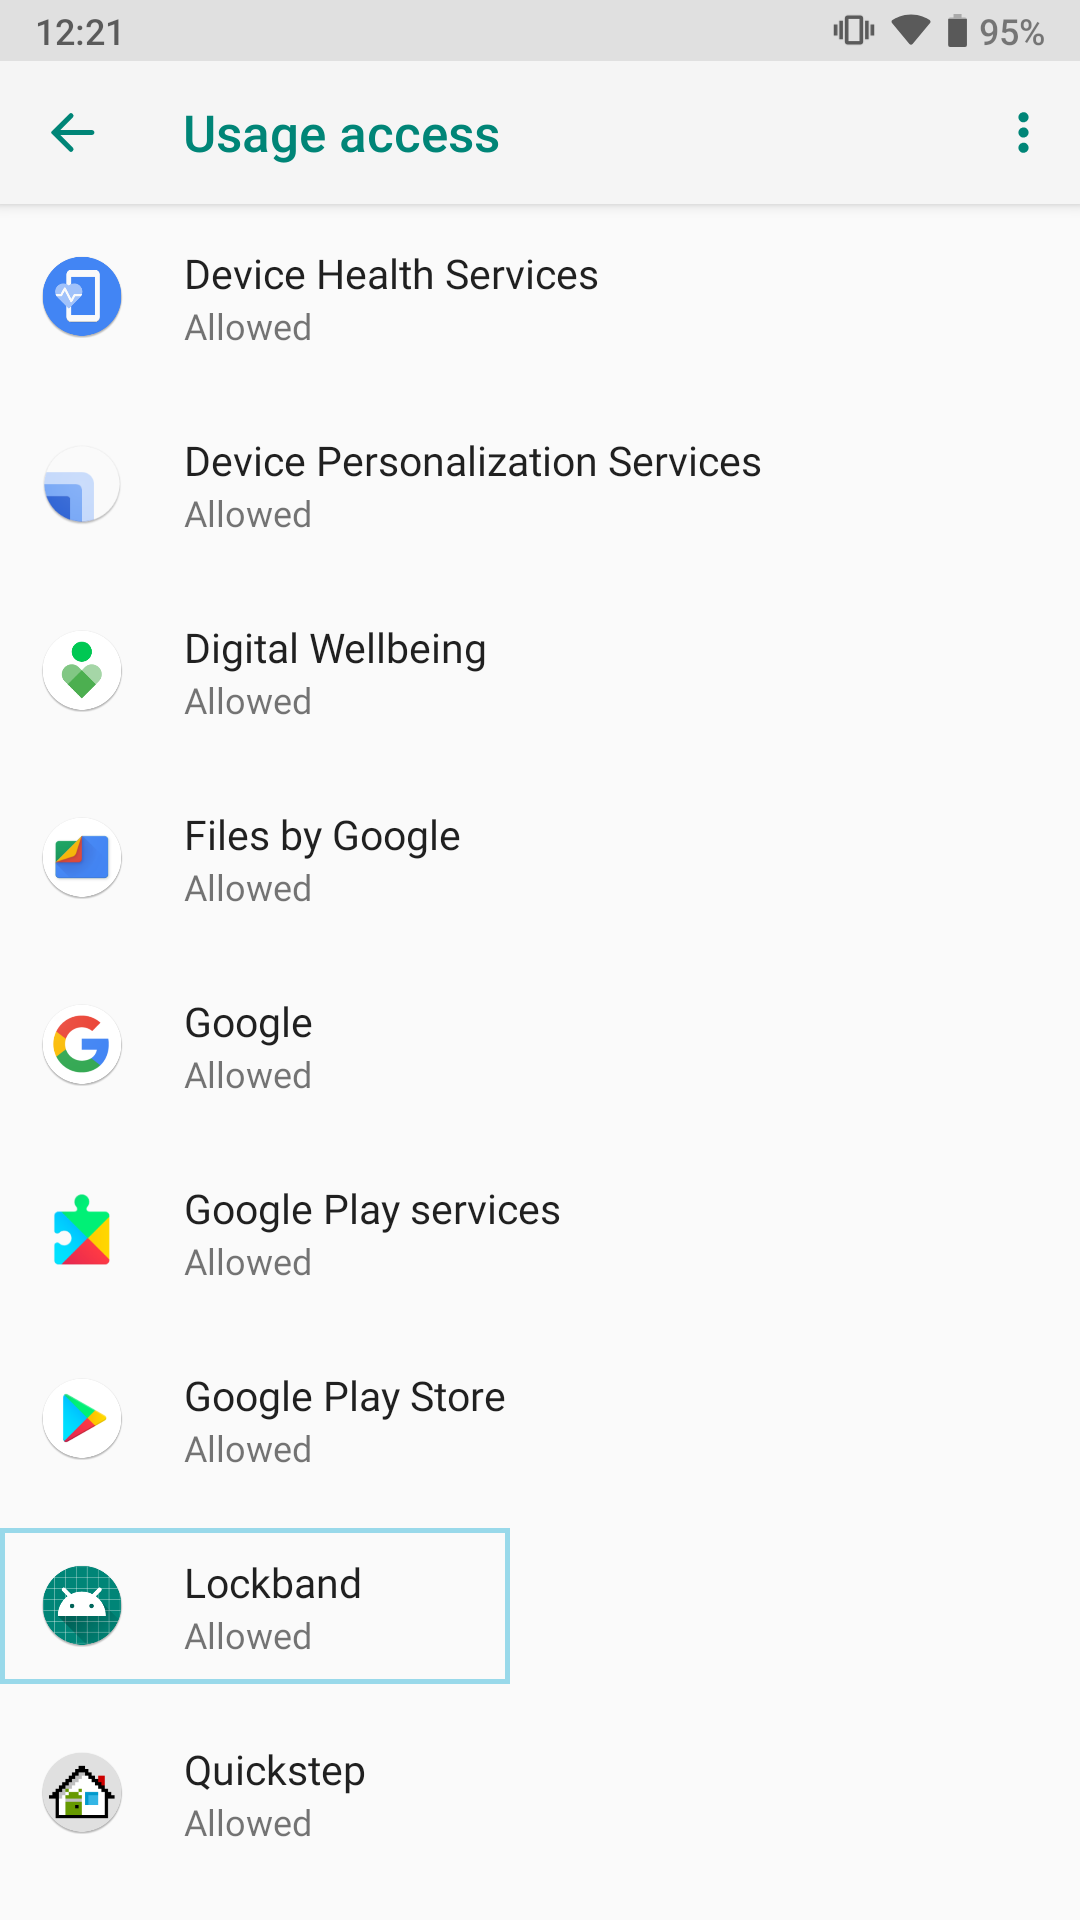
\includegraphics[width=0.3\textwidth]{app_screenshots/usage_stats_permission.png}
        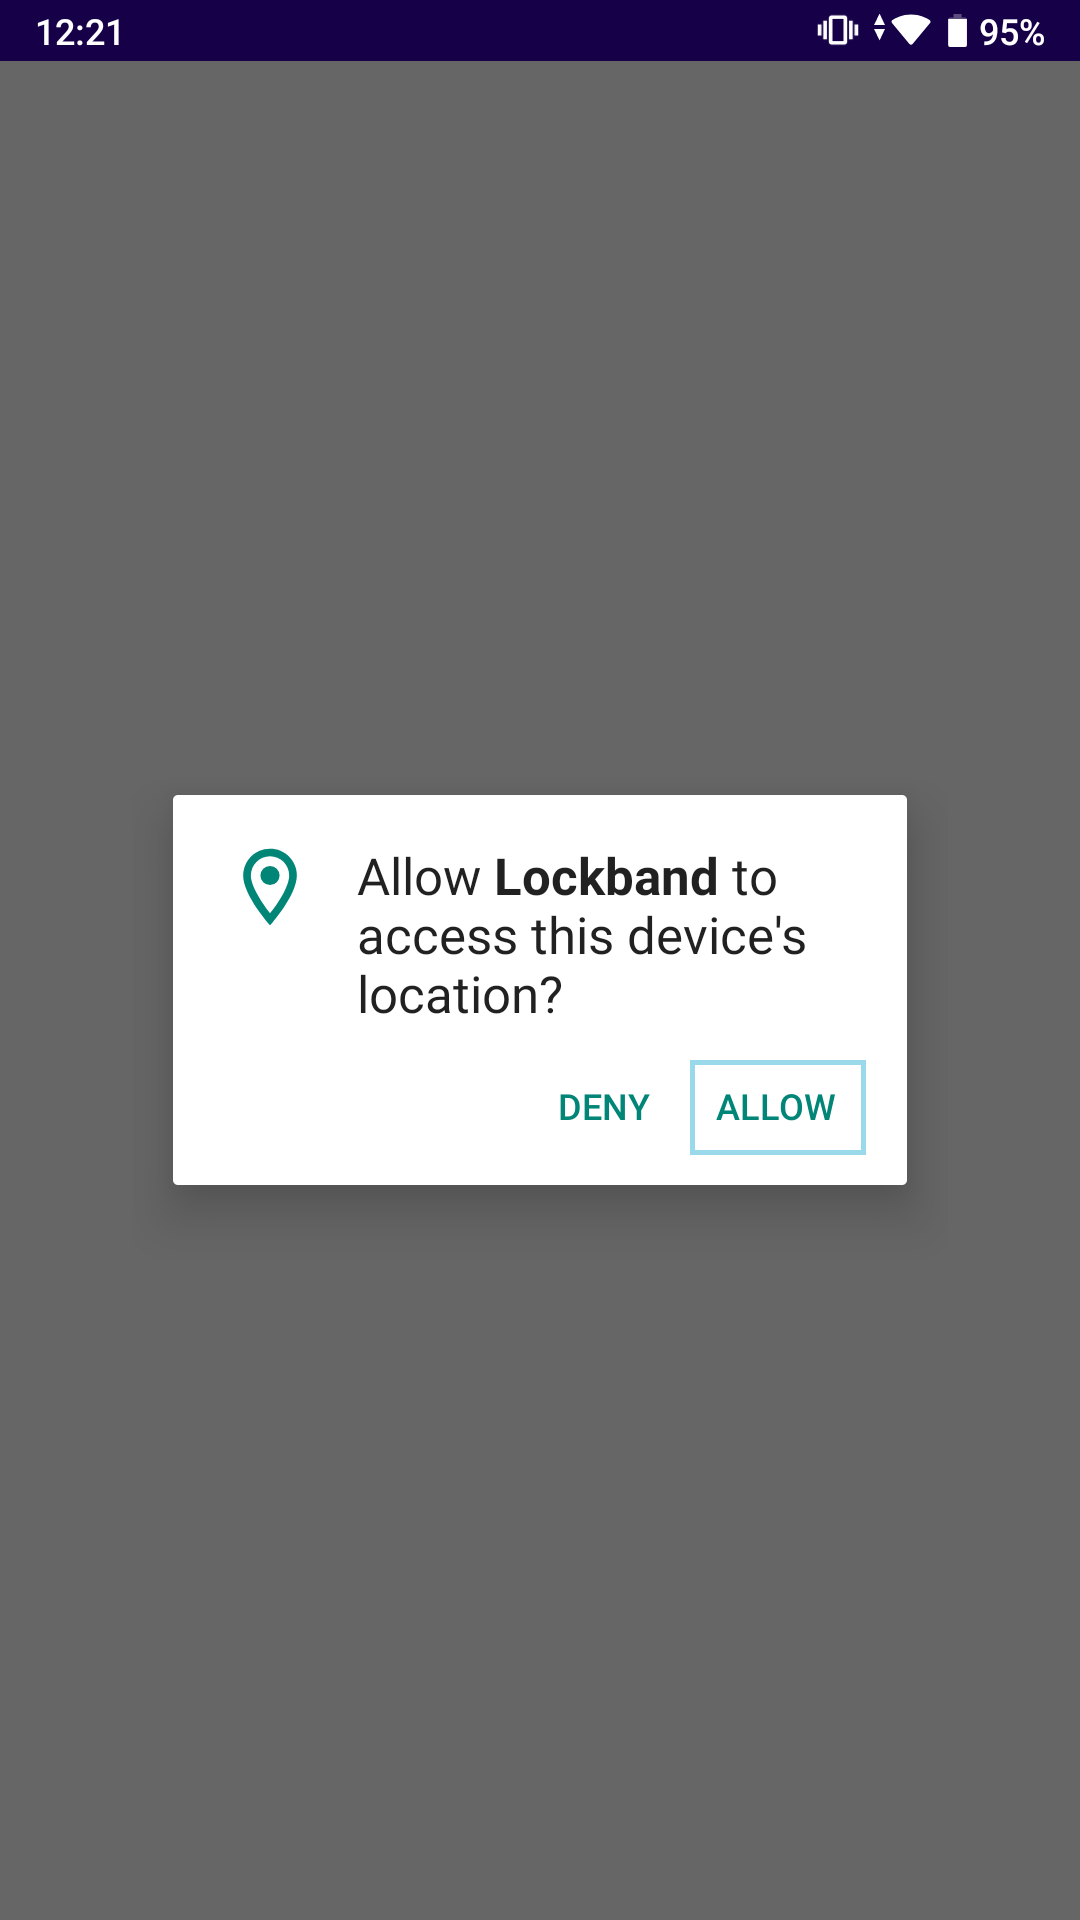
\includegraphics[width=0.3\textwidth]{app_screenshots/location_permission.png}
    \end{center}
    \caption{{\color{dgray}Udzielanie pozwoleń aplikacji}} \label{usageStats}
\end{figure}
Kolejnym etapem konfiguracji jest ustalenie hasła, które zostanie wykorzystane do odblokowania dostępu do chronionych aplikacji. Użytkownikowi zostaje wyświetlony formularz, w którym należy wprowadzić dwa identyczne hasła, a następnie zatwierdzić je przyciskiem poniżej. Wygląd formularza można zobaczyć w poniższej grafice.
\begin{figure}[H]
    \begin{center}
        \setlength{\fboxsep}{0pt}%
        \setlength{\fboxrule}{0.3pt}%
        \fbox{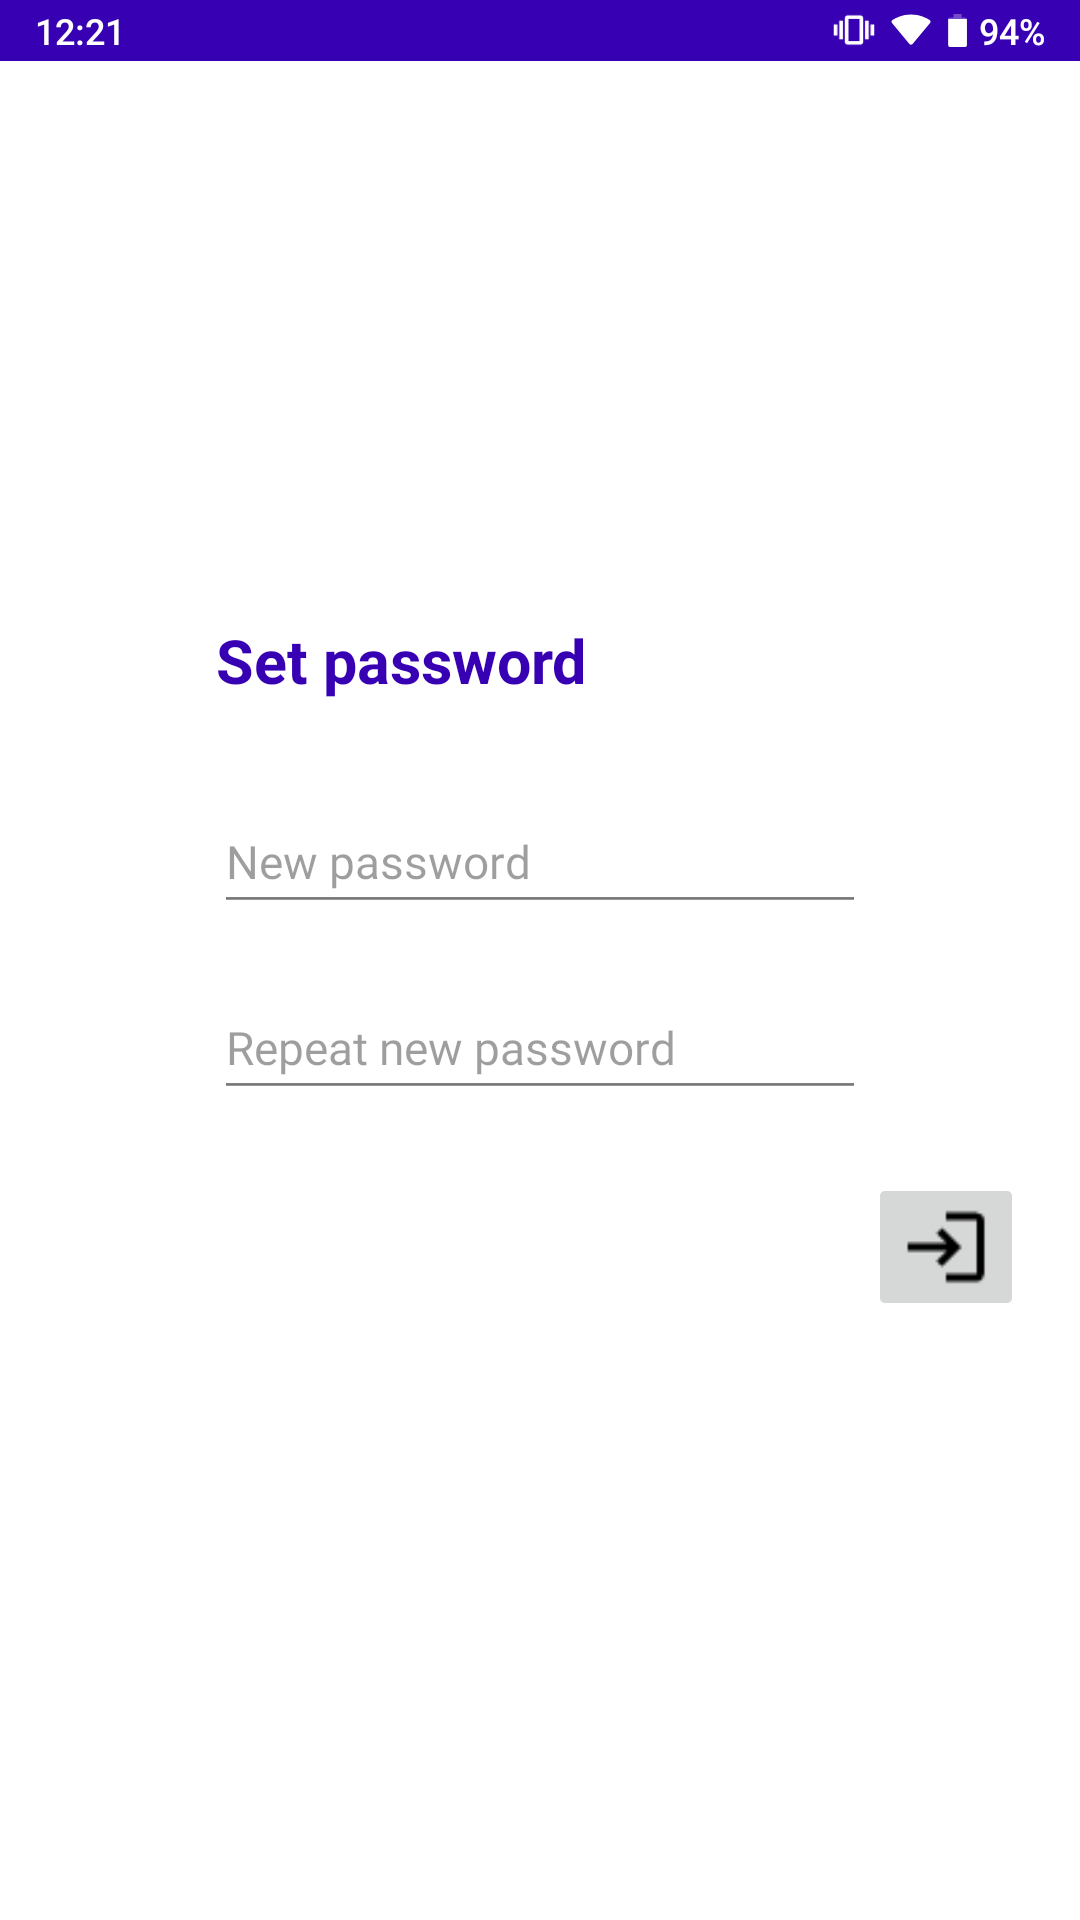
\includegraphics[width=0.3\textwidth]{app_screenshots/set_password.png}}
    \end{center}
    \caption{{\color{dgray}Formularz kreacji hasła}} \label{setPassword}
\end{figure}
Ostatnim etapem konfiguracji jest sparowanie opaski MiBand 3 z aplikacją. W tym celu zostaje wyświetlona aktywność odpowiedzialna za skanowanie pobliskich urządzeń Bluetooth. Po naciśnięciu przycisku \textit{Scan for devices} zostaje uruchomione skanowanie z nałożonym filtrem na typ urządzenia. Jeśli za pierwszym razem opaska nie zostanie znaleziona należy powtórzyć skan. Po znalezieniu urządzenia zostaje ono wyświetlone na liście. Aby rozpocząć proces parowania należy nacisnąć nazwę danego urządzenia. Po zakończeniu parowania konfiguracja dobiega końca i użytkownik zostaje przeniesiony do głównego menu aplikacji.
\begin{figure}[H]
    \begin{center}
        \setlength{\fboxsep}{0pt}%
        \setlength{\fboxrule}{0.3pt}%
        \fbox{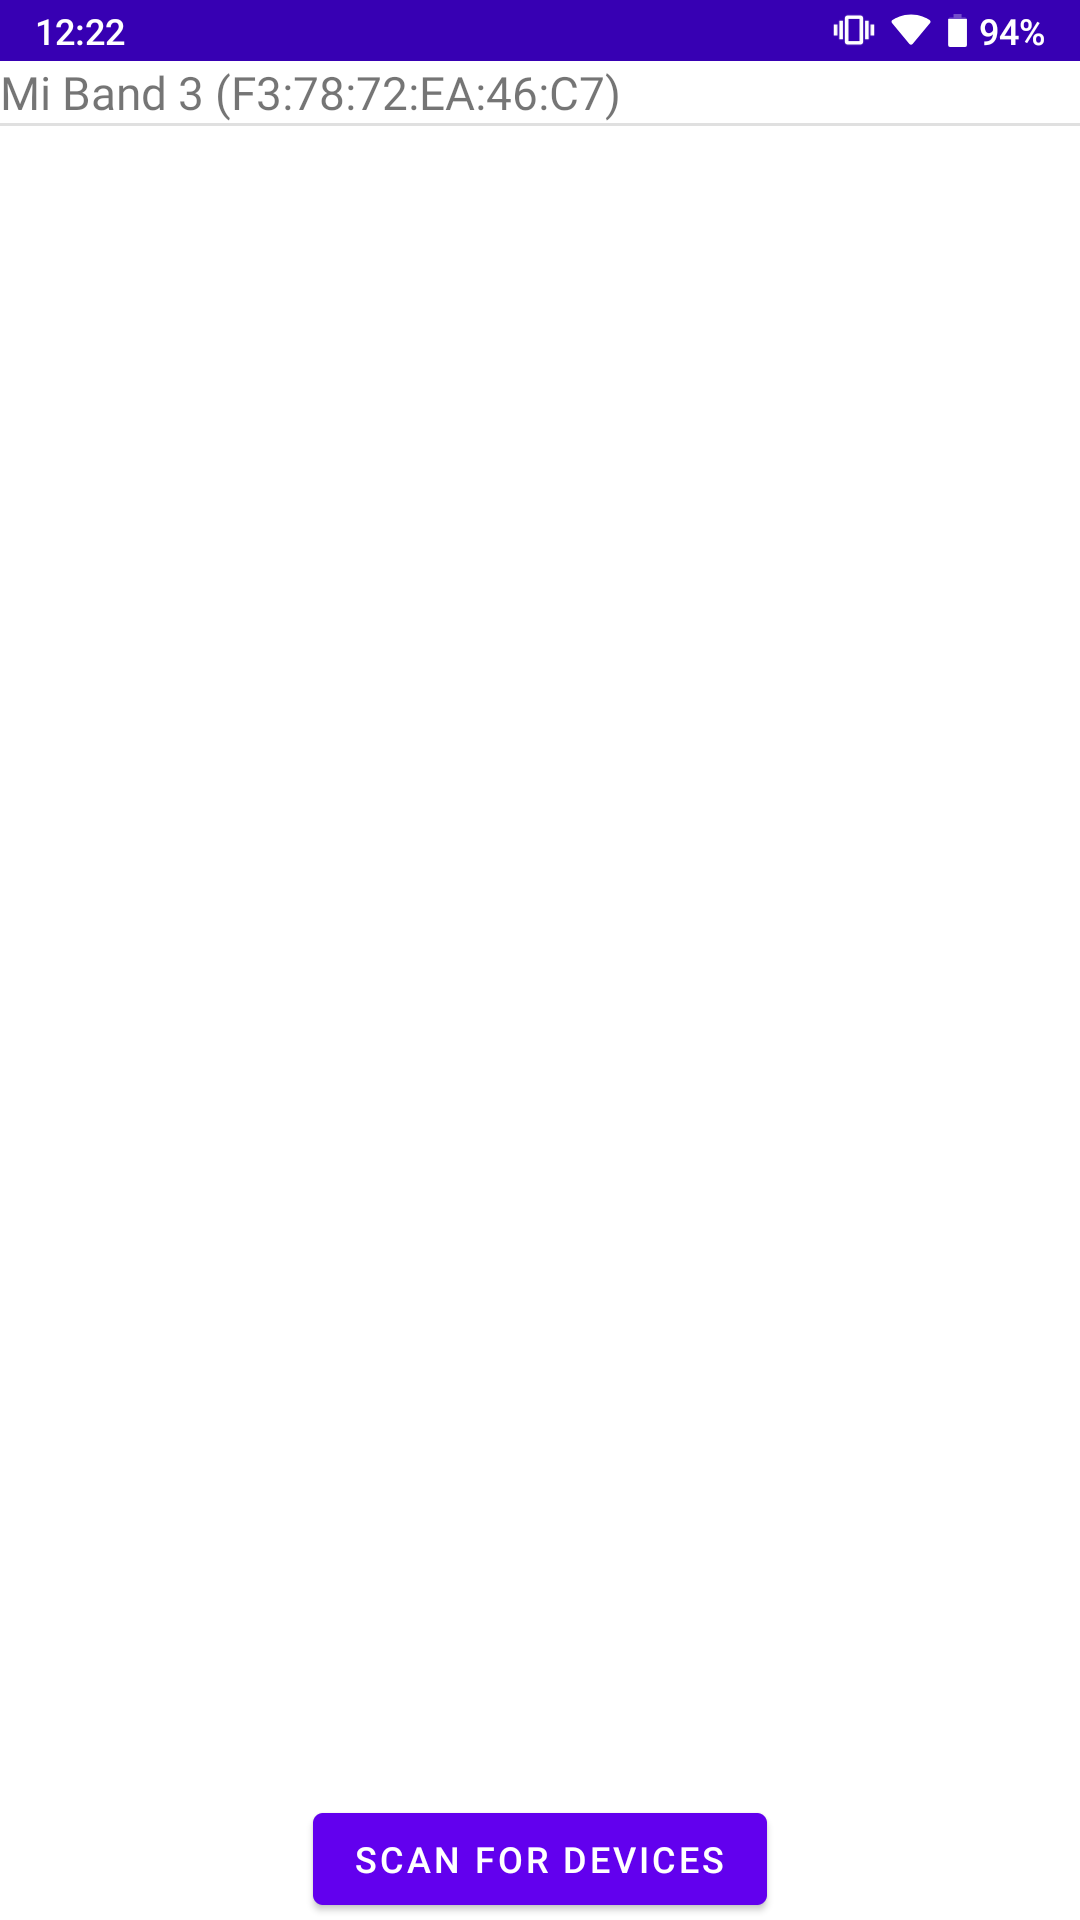
\includegraphics[width=0.3\textwidth]{app_screenshots/after_scan.png}}
    \end{center}
    \caption{{\color{dgray}Lista znalezionych po skanie opasek MiBand 3.}} \label{afterScan}
\end{figure}
\section{Przykłady użycia}
W tej sekcji przedstawię jak działa aplikacja od strony użytkownika poprzez opis czynności potrzebnych do wykonania określonych zadań, np. sprawdzenie stanu opaski, zmiana blokowanych aplikacji czy sprawdzenie statystyk.
\subsection{Wybór aplikacji do zablokowania}
\subsection{Zmiana hasła użytkownika}
\subsection{Wyświetlenie statystyk aktywności}
\subsection{Wyświetlenie informacji o opasce}
\subsection{Odblokowanie systemu}